% -*- mode: noweb; noweb-default-code-mode: R-mode; -*-









\graphicspath{ {datasets/} }


\chapter{Data Sets}
\label{cha:datasets}

This chapter presents summary descriptions of the various data sets
that are relevant to this analysis and further discussion on how they
were manipulated in preparation for analysis.  Operations where
multiple data sets are used in conjunction are deferred to Chapter
\ref{cha:analysis}.

The general approach with the MLCT and NLCD data sets is to reclassify
their categories, calculate per-pixel, per-class areas at the native
resolutions, and aggregate the new classification to the 5$'$ grid.
The purpose of the reclassification is to reduce the number of classes
and have a uniform set of classes across data sets.  The challenge in
this is that classification defintions are sometimes subtly different
which makes direct comparison across data sets somewhat subjective, so
we describe the mapping between original and simplified
classifications.  We apply and aggregation operation that calculates
the relative proportion of each class in the new classification system
present in each 5$'$ grid cell according to the base data.  In this
process we convert classified maps whose pixels have discrete values
to a stack of maps, one map per class, whose pixels have real number
values on the interval $[0,1]$ representing fractional areas and are
constrained to sum to unity for each pixel through the stack.  In the
general case of the MLCT data product the process converts two
discrete, thematic variables and one continuous variable, those being
a primary covery type, a secondary cover type, and classification
confidence level respectively, into a set of continuous variables
representing fractional areas for the cover types in the siplified
classification system.  This general case is also compared to simpler
cases of the NLCD and considering only the primary classification of
MLCT.  In these cases the process is simplified by considering only a
primary thematic layer and performing the aggregation without a
secondary cover type or confidence level by which to relate them but
we are able to reuse the same functions for the raster calculations.

To illustrate the process of converting the these data sets from their
original representation we are including maps of an area of
southeastern Michigan to show greater detail through each step of the
process.  We chose this region for its diversity of land covers and
uses, its relative diveristy of agricultural commodities across its
significant cropland area, the significant presence of the mosaic
class to illustrate our method for its decomposition and its
familiarity to our principal author, being his brthplace.


\section{MODIS Land Cover Type (MLCT)}
\label{sec:mlct}

In preparation for this analysis we prepared the 2001 MLCT data by
patching together the tiles as delivered in the equal-area sinusoidal
projection, reprojecting that mosaic to geographic coordinates, and
extracting a subset for the conterminous United States (cUSA).  These
preparation steps were carried out in a \texttt{GRASS} database prior
to the adoption of the reproducible research framework for this paper,
so those steps are not demonstrated here.  The cUSA study area is
defined as the set of 5$'$ grid cells that intersect with the cUSA
polygon in version 1 of the Global Administrative Areas (GADM) vector
data set, which includes the water bodies on the American side of the
international border across the Great Lakes, but does not extend to
oceanic waters beyond the coastal grid cells that intersect with any
land mass.

In this section we will demonstrate the process of converting the MLCT
data from its native form, consisting of primary cover type,
classification confidence for the primary cover, and secondary
(alternate) cover type at 15$''$ resolution, to a stack of cover
fractions at 5$'$ resolution using the simplified cover/use
classification specified by the PEEL model.

\subsection{Reclassification}
\label{sec:mlct-reclass}

The following table shows the mapping of the IGBP classes used in the
original MLCT data to the simplified classification designed for the
PEEL model.

\begin{center}
  \begin{table}[htbp]
    \begin{tabular}{|l|l|l|l|}
      \hline
      \multicolumn{2}{|c|}{MLCT/IGBP} & \multicolumn{2}{|c|}{PEEL} \\
      \hline
      0 & water & 0 & water \\
      \hline
      1 & evergreen needleleaf forest & \multirow{5}{*}{1} & \multirow{5}{*}{forest} \\
      2 & deciduous needleleaf forest & & \\
      3 & evergreen broadleaf forest & & \\
      4 & deciduous broadleaf forest & & \\
      5 & mixed forests & & \\
      \hline
      6 & closed shrublands & \multirow{3}{*}{2} & \multirow{3}{*}{shrub} \\
      7 & open shrublands & & \\
      8 & woody savannas & & \\
      \hline
      9 & savannas & \multirow{2}{*}{3} & \multirow{2}{*}{open} \\
      10 & grasslands & & \\
      \hline
      11 & permanent wetlands & 4 & wetland \\
      \hline
      12 & croplands & 5 & crop \\
      \hline
      13 & urban & 6 & urban \\
      \hline
      14 & cropland / natural vegetation mosaics & 7 & mosaic \\
      \hline
      15 & permanent snow and ice & \multirow{2}{*}{8} & \multirow{2}{*}{barren} \\
      16 & barren or sparsely vegetated & & \\  
      \hline
    \end{tabular}
    \caption{Reclassification of MLCT/IGBP to PEEL}
    \label{tab:mlct_reclass}
  \end{table}
\end{center}




\begin{figure}[hpt] 
  \centering
  

\includegraphics{fig_thumb_pri_reclass}
%\end{center} 
\caption{MLCT primary cover reclassified detail} 
\label{fig:thumb_pri_reclass} 
\end{figure} 

\todo{Is this figure any better placed than others?}

\autoref{fig:thumb_pri_reclass} shows the result of reclassifying the MLCT data
for our detailed study area.  From this map we see that this area is
dominated by the crop class in the north and the mosaic class to the
south with scattered forests and pockets of development throughout.
The urban complex of Port Huron, Michicagn and Sarnia, Ontario is
visible in the southeast corner.  along with the confidence level given for
the primay classification.

\begin{figure}[hpt] 
\begin{center}
  

\includegraphics{fig_thumb_sec_reclass}
\end{center} 
\caption{MLCT secondary cover reclassified detail} 
\label{fig:thumb_sec_reclass} 
\end{figure} 


In \autoref{fig:thumb_sec_reclass} we notice that areas in the
northern and central sections of the map that were classified as crop
in the primary layer have null values in the secondary class.  It is
apparent that where a secondary class is given that the mosaic class
is often indicated where the primary class indicates cropland and vice
versa.  It is possible for primary and secondary classes to be
assigned to the same category because of the reclassification step.
When one of our pixels indiactes the forest class for both its primary
and secondary classifications it simply reflects a distinction between
sub-types of forest in the original data, for example evergreen and
deciduous.

\begin{figure}[hpt] 
\begin{center}
  

\includegraphics{fig_thumb_pct}
\end{center} 
\caption{MLCT primary cover classification confidence} 
\label{fig:thumb_pct} 
\end{figure} 

\autoref{fig:thumb_pct} shows the confidence level as a percentage.
We see that the areas where no secondary class is given are areas
where confidence is 100\% and the primary classification is cropland
and therefore would be accounted as 100\% cropland by area by any
method of adding up these areas.  In light of this observation it is
clear that MLCT will generally over-estimate cropland because it is
certain that these areas are not completely under cultivation but
rather are interspersed with homesteads, fence lines, small wood lots,
roads, and such cultural features.  In areas such as this that were
made available for settlement in the 19th century according to the
Public Land Survey System (PLSS) we expect to find roads delineating
every square mile in general.  

The relationships described among the three layers of the MLCT are
perhaps more easily appreciated visually by mapping the individual
classes separately.  \autoref{fig:thumb_pri_facet} does this for the
primary class in our example detail area and
\autoref{fig:thumb_sec_facet} for the secondary class.


\begin{figure}[hpt] 
\begin{center}
  

\includegraphics{fig_thumb_pri_facet}
\end{center} 
\caption{MLCT primary covers shown separately, detail} 
\label{fig:thumb_pri_facet} 
\end{figure} 


\begin{figure}[hpt] 
\begin{center}
  

\includegraphics{fig_thumb_sec_facet}
\end{center} 
\caption{MLCT secondary covers shown separately, detail} 
\label{fig:thumb_sec_facet} 
\end{figure} 

%\subsubsection{Analysis Area}
%\label{sec:reclass-analysis-area}

Conveniently we are able to reuse the same functions for
reclassification and mapping of the data that we have prepared for the
larger study area.  \autoref{fig:mlct_pri_reclass} shows the map of
the primary classification across the cUSA, and likewise
\autoref{fig:mlct_sec_reclass} for the secondary layer and
\autoref{fig:mlct_pct} for the confidence level.  Because the maps are
showing a greater extent in relatively the same amount of page space
it is even more useful to create the facet maps for the individual
classes as \autoref{fig:mlct_pri_facet} and
\autoref{fig:mlct_sec_facet} have done.  From these maps familiar
generalities of the cUSA's geography are more apparent, such as the
prevalence of forests in the east and northwest, cropland in the
midwest, shrub lands in the southwest and open lands across the west.
It is interesting to note that the mosaic class is primarily
concentrated in the eastern portion of the study area which we can
attribute to greater population density, topography, and historical
patterns of settlement resulting in characteristically smaller parcels
and a greater degree of mixing among agricultural uses and natural
covers.



\begin{figure}[hpt] 
\begin{center}


\includegraphics{fig_mlct_pri_reclass_trim}
\end{center} 
\caption{MLCT primary cover reclassified} 
\label{fig:mlct_pri_reclass} 
\end{figure} 

\todo{Make cUSA graphics wider or even turn sideways for full-page}

\begin{figure}[hpt] 
\begin{center}
  

\includegraphics{fig_mlct_sec_reclass_trim}
\end{center} 
\caption{MLCT secondary cover reclassified} 
\label{fig:mlct_sec_reclass} 
\end{figure} 


\begin{figure}[hpt] 
\begin{center}
  

\includegraphics{fig_mlct_pct_trim}
\end{center} 
\caption{MLCT primary cover classification confidence} 
\label{fig:mlct_pct} 
\end{figure} 


\begin{figure}[hpt] 
\begin{center}
  

\includegraphics{fig_mlct_pri_facet}
\end{center} 
\caption{MLCT primary covers shown separately} 
\label{fig:mlct_pri_facet} 
\end{figure} 

\todo{ Split \autoref{fig:mlct_pri_facet} into two figures.}

\begin{figure}[hpt] 
\begin{center}
  

\includegraphics{fig_mlct_sec_facet}
\end{center} 
\caption{MLCT secondary covers shown separately} 
\label{fig:mlct_sec_facet} 
\end{figure} 

\todo{ Split \autoref{fig:mlct_sec_facet} into two figures.}

\subsection{Aggregation}
\label{sec:mlct-aggr}

MLCT has a nominal resolution of 500m which roughly equates to 15$''$
at the eqautor and so is conveniently an even division of the 5$'$
grid to which we wish to aggregate it, the two related by a factor of
20.  Therefore each cell in the output of this aggregation will be a
function of the 400 orginal MLCT pixels within its footprint.  The
dataset consists of a primary classification, along with a measure of
confidence up to 100\%, and a secondary classification.  The secondary
cover type is given as the most likely alternative to the primary type
\citep{Friedl2010}, but for purposes of our analysis we are taking a
more probabilistic view and incorporating all available information
from the base data.  We are not as concerned about per-pixel
classification error as users working at the MLCT's native resolution
might be, which is the original motivation given for providing the
secondary classification.  Because we are aggregating the data up to
5-arcmin resolution there is no expectation that the sub-pixel
fractions at full resolution are spatially specific, but in the
aggregate our characterization of each grid cell's composition will be
nuanced by this additional information.  The primary class covers at
least roughly 50-60\% of a given pixel $x$, and this percent is almost
certainly a monotonically increasing function of the confidence
measure $c$.  \todo{cite email from Friedl}.  For the purposes of this
analysis we assume that this dependence is linear. Thus, for the
primary and secondary cover types in a pixel:

$$
A_p(x) = A_{min} + (1 - A_{min}) c(x)
$$
$$
A_s(x) = 1 - A_p(x)
$$

where $0.50 \le A_{min} \le 0.60$ is primarily chosen based on an
interpretation of $c$.  Given that there are only a handful of
examples of $c < 0.20$ \todo{consider including histograms showing
  confidence distribution}, setting $A_{min} = 0.50$ is appropriate.
Certainly for a classification to be considered the primary it must
represent a bare majority of the area covered by that pixel at
minimum, and the distributions of confidences indicate that the vast
majority of pixels contain greater than 60\% of their area in the
primary under the rubric described above.  The equations are simplified
as follows by assuming this value for $A_{min}$.

$$
A_p(x) = \dfrac{1 + c}{2}
$$
$$
A_s(x) = 1 - A_p(x) = \dfrac{1-c}{2}
$$

% will this help?



Applying these formulae results in a map for each cover type where the
pixel values are the sub-pixel areas on the interval $[0,1]$.  The map
of the fraction of the primary cover type is visually equivalent to
that of the classification confidence level because the former is
simply a linear scaling and offset of the latter.  \autoref{fig:thumb_fracs} shows the result of calculating $A_p + A_s$ for each individual class.  

%\subsubsection{Detail Area}
%\label{sec:agg-detail-area}


\begin{figure}[hpt] 
\begin{center}
  

\includegraphics{fig_thumb_fracs}
\end{center} 
\caption{Sub-pixel fractions at original resolution for $A_{min}=0.5$}
\label{fig:thumb_fracs}
\end{figure} 

By way of comparison we also consider the trivial case of settimg
$A_{min} = 1$ which indicates that the secondary cover is ignored
altogether and the primary cover is taken to represent 100\% of the
pixel area.  \autoref{fig:thumb1_fracs} shows these difference.  The
effect of adjusting $A_{min}$ is subtle; we will examine it more
closely after aggregating to the 5$'$ grid.

\begin{figure}[hpt] 
\begin{center}


\includegraphics{fig_thumb1_fracs}
\end{center} 
\caption{Sub-pixel fractions at original resolution for $A_{min}=1$}
\label{fig:thumb1_fracs}
\end{figure} 

Computationally the process of converting the reclassified maps to
sub-pixel fractions at the desired 5-arcmin resolution is a three-step
process.  First we calculate the fraction of the primary cover type as
a function of the classification confidence as described above.  Next,
a sub-pixel fraction for each cover type is calculated at full
resolution, recognizing that the primary and secondary classes may be
identical after the reclassification, such as cases where the original
data indicated two different type of forests.  Aggregating to a
coarser resolution is a simple matter of calculating the mean of these
values over the intersecting pixels at the original resoution.
Because the desired 5$'$ resolution is a multiple of the original
15$''$ resolution the pixels are perfectly nested, which is
convenient for properly computing this mean.


\begin{figure}[hpt] 
\begin{center}
  

\includegraphics{fig_thumb_agg}
\end{center} 
\caption{Aggregated sub-pixel fractions for $A_{min}=0.5$}
\label{fig:thumb_agg}
\end{figure} 

\begin{figure}[hpt] 
\begin{center}
  

\includegraphics{fig_thumb1_agg}
\end{center} 
\caption{Aggregated sub-pixel fractions for $A_{min}=1$}
\label{fig:thumb1_agg}
\end{figure} 


Before proceeding further it is interesting to inspect the differences
between the aggregated maps for the chosen values of $A_{min}$ as
shown in \autoref{fig:thumb_agg_diff}.  Positive values indicate that
$A_{min} = 0.5$ resulted in a greater fraction.  The main message from
this chart is that considering the secondary cover class results in
greater mixture between the crop and mosaic classes because cropland
is reduced in the north of the detail area where it was dominant in
the primary land cover type, and simlarly for mosaic in the south.
The relative suitability of these choices for $A_{min}$ is discussed
in \autoref{cha:analysis}.



\autoref{fig:thumb_agg_diff} emphasizes the difference between the
choice of $A_{min}=0.5$ and $A_{min}=1.0$ for the calculation of the
sub-pixel fractions and their aggregation to 5$'$ with a difference
map.  Positive values in the map indicate areas where $A_{min}=0.5$
produced a greater value.  We see more clearly from this set of maps
that the effect of considering the secondary class results in a shift
of up to 10\% of total cell area from crop to mosaic in the north of
our detail area and vice versa for the southern portion.  This
decrease in the relative dominance of the primary class is expected as
we saw from the earlier maps (\autoref{fig:thumb_pri_facet} and
\autoref{fig:thumb_sec_reclass}) of the MLCT data which classes were
indicated by the secondary classes in those areas.

\begin{figure}[hpt]
\begin{center}
  
%def

\includegraphics{fig_thumb_agg_diff}
\end{center} 
\caption{ Difference of aggregated sub-pixel fractions}
\label{fig:thumb_agg_diff}
\end{figure} 

%\subsubsection{Analysis Area}
%\label{sec:agg-analysis-area}


We apply the same functions for calculating the $15''$-resolution map
of the primary cover class as a function of the confidence level $c$
for the entire cUSA study area, converting those to per-class
fractions at the same extent and scale, and aggregating those values
to the $5'$ grid.  The corresponding figures are not shown because the
decrease in relative resolution makes interpretation difficult.  Based
on the behavior that these functions exhibited over the detail area we
can be confident that they will perform correctly over the greater
extent.



\subsection{Mosaic decomposition}
\label{sec:decomposition}

The MLCT classification includes a type that is problematic for the
economic models for which this data set is intended, the ``cropland /
natural vegetation mosaic'' class.  This class is defined as a hybrid
of cropland and some mixture of natural covers (forest, shrub, or
open) with no single component exceeding 60\% \citep{Friedl2002} and
croplands generally comprising 40--60\% of pixel area \todo{cite Friedl
  email}. Being a hybrid of developed land use and natural land cover
we wish to differentiate the cropland from the natural vegetation in
order to calculate a more meaningful total for cropland area and
thereby eliminate the mosaic class from the final tabulation.  In the
present implementation of the reclassification and aggregation process
we are making three very simple assumptions about the composition of
area delineated as mosaic lands:

\begin{enumerate}
\item Mosaic land is 50\% cropland.
\item The other 50\% is a blend of forest, open, and shrub in
  proportion to the expression of those classes in the same 5-minute
  cell.
\item In the absence of such information we simply assume that the
  natural component of the mosaic is an equal blend of all three.
\end{enumerate}

The intention here is to make simplifying assumptions that will allow
us to proceed with the evaluation of this analytical framework.
Although it may be interesting to vary the proportion used to
calculate the proportion of mosaic land to be allocated to crop land
we have no principled basis for this as of yet, considering that the
defintion implies that this proportion is variable across the MLCT
rather than being some unknown single-valued quantity.  The choice of
the 50\% level reflects the assertion that the mosaic is a cultural
class grouped with cropland and urban in the IGBP classification
scheme without overstating the degree of development.  MLCT provides
adequate variability in this dimension by commonly pairing cropland
and mosaic in the primary/secondary class data.  The second assumption
imposes that 15$''$ mosaic cells' non-crop portion will have the same
relative composition of forest, open, and shrub as the as the
non-mosaic portion of the 5$'$ grid cell in which it falls. Therefore
mosaic pixels in a 5$'$ cell where only forest is found of the three
non-crop mosaic components will be allocated 50\% crop and 50\%
forest.  \autoref{fig:thumb_nomos} and \autoref{fig:thumb1_nomos} show
the effect of decomposing the mosaic class in this fashion for
$A_{min}$ values of 0.5 and 1.0 respectively.



\begin{figure}[hpt]
\begin{center}
  


\includegraphics{fig_thumb_nomos}
\end{center} 
\caption{Aggregated cover fractions after mosaic decomposition, $A_{min}=0.5$}
\label{fig:thumb_nomos}
\end{figure} 

\begin{figure}[hpt]
\begin{center}
  


\includegraphics{fig_thumb1_nomos}
\end{center} 
\caption{Aggregated cover fractions after mosaic decomposition, $A_{min}=1.0$}
\label{fig:thumb1_nomos}
\end{figure} 



\begin{figure}[hpt]
\begin{center}
  

\includegraphics{fig_thumb_nomos_diff}
\end{center} 
\caption{Differences of sub-pixel fractions after mosaic
  decomposition, positive when $f(A_{min} = 0.5)$ is greater}
\label{fig:thumb_nomos_diff}
\end{figure} 





Our hypothesis from the outset is that there is information worth
capturing in the secondary class and classification confidence level
provided by MLCT.  We will test this hypothesis in
\autoref{cha:analysis} but in order to do so we need an ``observed
truth'' to provide an independent standard by which to make a
comparison on the basis of overall reduction in error at the 5$'$ grid
cell level.  The following section describes such a data set which
will be held up against these MLCT-derived data sets in the next
chapter.

% more appropriately addressed in following chapter

% Both 5-arcmin data sets derived from the MLCT in this fashion
% overestimate cropland area relative to that indicated by Agland2000,
% but the $A_{min} = 0.5$ variant better portrays the spatial variation
% judging from a simple root-mean-squared-error (RMSE)
% test. \todo{illustrate/demonstrate the RMSE test on the 5-arcmin MLCT
%   data sets}



\section{National Land-cover Database 2001 (NLCD)}
\label{sec:nlcd}


The NLCD gives a higer-resolution (30m) snapshot of LULC circa 2001.
Because NLCD's classification was informed by ancillary data sets such
as population density, buffered roads, and the National Wetland
Inventory \citep{Homer2004} reclassifying and aggregating this data to
5-arcmin resolution in a fashion similar to that used for the MLCT is
expected to give better estimations of aggregate area for detailed
features like rural transportation networks and small stream and
wetland features.  This is supported by the statment in
\citet{Homer2007} that part of the NLCD post-processing algorithm was
designed ``to allow non-linear features like roads and streams to
remain intact.''  Although it is unclear from \citet{Homer2004} what
ancillary data was applied in what consituent mapping zones of the
NLCD we accept its representation of these fine details to be the best
available data.  This will compensate for MLCT's bias against these
finely detailed structures due to it's resolution.  It is the
availability of this information that makes it difficult to apply this
analysis beyond the United States without access to a comparable data
set with global extents.  The analysis is restricted to the
conterminous US because of the relative paucity of agricultural
activity in Hawaii and Alaska.

As with the MLCT the process of reclassification and aggregation is
performed for both the detail region and the complete region.

One limitation of the \texttt{raster} library for \texttt{R} that we
are using is that the aggregation function requires that the output
resolution be a multiple of the output resolution.  The 30m resolution
of the NLCD equates to 1.25361$''$ and so does not satisfy this
requirement.  This deficiency was addressed by resampling the input to
1.25$''$ resolution prior to export from \texttt{GRASS} for this
analysis using a nearest-neighbor sampling algorithm, which gives an
even factor of 240 between the two resolutions.

\todo{Incorporate Joshua's suggestion to show further NLCD detail to better illustrate the discrepancy in developed areas}


\subsection{Reclassification}
\label{sec:nlcd-reclass}


\begin{center}
  \begin{table}[htbp]
    \begin{tabular}{|l|l|l|l|}
      \hline
      \multicolumn{2}{|c|}{NLCD} & \multicolumn{2}{|c|}{PEEL} \\
      \hline
      11 & water & \multirow{3}{*}{0} & \multirow{3}{*}{water} \\
      98 & palustrine aquatic bed* & & \\
      99 & estuarine aquatic bed* & & \\
      \hline
      41 & deciduous forest & \multirow{3}{*}{1} & \multirow{3}{*}{forest} \\
      42 & evergreen forest & & \\
      43 & mixed forest & & \\
      \hline
      52 & shrub / scrub & \multirow{2}{*}{2} & \multirow{2}{*}{shrub} \\
      94 & estuarine scrub / shrub wetland & & \\
      \hline
      71 & grassland / herbaceous & \multirow{2}{*}{3} & \multirow{2}{*}{open} \\
      81 & pasture / hay & & \\
      \hline
      90--93 & woody wetlands & \multirow{2}{*}{4} & \multirow{2}{*}{wetland} \\
      % 91 & palustrine forested wetland* & & \\
      % 92 & palustrine scrub/shrub wetland* & & \\
      % 93 & estuarine forested wetland* & & \\
      % 94 & estuarine scub/shrub wetland* & & \\
      95--97 & emergent herbaceous wetlands & & \\
      % 96 & palustrine emergent wetland (persistent)* & & \\
      % 97 & palustrine scrub/shrub wetland* & & \\
      \hline
      82 & cultivated crops & 5 & crop \\
      \hline
      21 & developed, open space & \multirow{4}{*}{6} & \multirow{4}{*}{urban} \\
      22 & developed, low intensity & & \\
      23 & developed, medium intensity & & \\
      24 & developed, high intensity & & \\
      \hline
       & (no equivalent) & 7 & mosaic \\
      \hline
      12 & perennial ice/snow & \multirow{2}{*}{8} & \multirow{2}{*}{barren} \\
      31 & barren land & & \\  
      32 & unconsolidated shore & & \\  
      \hline
    \end{tabular}
    \caption{Reclassification of NLCD to PEEL}
    \label{tab:mlct_reclass}
  \end{table}
\end{center}


\begin{figure}[hpt] 
\begin{center}


\includegraphics{fig_thumb_nlcd_reclass}
\end{center} 
\caption{NLCD reclassified} 
\label{fig:thumb_nlcd_reclass} 
\end{figure} 

\begin{figure}[hpt] 
\begin{center}
  

\includegraphics{fig_thumb_nlcd_facet}
\end{center} 
\caption{NLCD covers shown separately, detail} 
\label{fig:thumb_nlcd_facet} 
\end{figure} 

\subsection{Aggregation}
\label{sec:nlcd-aggr}

The same code used for refactoring the MLCT when considering only the
primary cover type can be applied here.

Repeating this process for the entire study area is computationally
expensive due to the NLCD's high resolution.


 

\begin{figure}[hpt] 
\begin{center}
  


\includegraphics{fig_thumb_nlcd_agg}
\end{center} 
\caption{NLCD aggregated cover fractions, detail area}
\label{fig:thumb_nlcd_agg}
\end{figure} 

\todo{ Split \autoref{fig:mlct_nlcd_agg} into two figures.}


\begin{figure}[hpt] 
\begin{center}
  


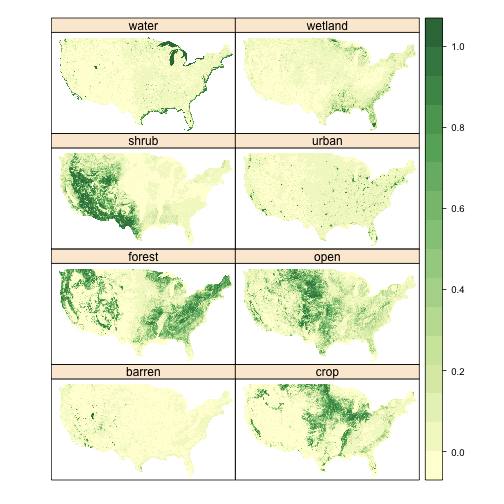
\includegraphics{fig_nlcd}
\end{center} 
\caption{NLCD aggregated cover fractions}
\label{fig:nlcd}
\end{figure} 

\begin{comment}
\section{Cropland Data Layer (CDL)}
\label{sec:cdl}

\missingfigure{Table or chart showing CDL covereage for various years}

The CDL is only available for a small number of states in 2001.  If
time allows it might be good to compare what is available with our
results as another independent evaluation against a higher-resolution
data set.

\subsection{Reclassification}
\label{sec:cdl-reclass}



%  gdalbuildvrt -tr 0.0002777778 0.0002777778 -te -124.8333 24.5 -66.91667 49.33333 cdl_2001.vrt $(find . -name "*2001*")


\todo{Calculate CDL mask for 5-arcmin cells completely filled}
\todo(Calculate CDL aggregated in GRASS}




\missingfigure{CDL reclassification table}

\subsection{Aggregation}
\label{sec:cdl-aggr}
\end{comment}

\section{Agricultural Lands in the Year 2000 (Agland2000)}
\label{sec:agland2000}


The data set described by \citet{Ramankutty2008}, referred to in this
paper as ``Agland2000'', is the product of an effort to merge
satellite-derived LULC classifications with census data of arable land
and permanent crops compiled at national or sub-national levels
according to availability of such data at or near the turn of the last
century.  It uses two classified LULC data sets derived from remote
sensing data as inputs, an older version of the MLCT (known as
BU-MODIS) and the GLC2000 data set mentioned in
\autoref{sec:background}.  Its allocation of cropland and pastures is
constrained by a mask based on climatic criteria in order tp avoid
misallocation at higher latitudes, mainly a problem in boreal Canada
which should have little to no bearing on our study area.  The
``open'' class in this data set has been renamed from ``pasture'' in
its creator's nomenclature, but it is clear from its distribution
shown in \autoref{fig:agland} that it represents a phenomena that is
not apparent in the MLCT data, so we do not attempt to use it or
reconcile it here, rather only carry it along to a small degree for
sake of comparison.  We attribute this discrepancy to commingling of
managed pasture lands and natural open land in the MLCT
classification.  It is important to note that Agland2000 is used as an
input into the classification algorithm of the version of MLCT that we
are using here and acknowledge the possibility of circularity when
comparing the two, but because of its basis in census data we will use
the cropland component of Agland2000 as an ``observed truth'' for the
purposes of evaluating our incremental adjustments to the maps we
derive from MLCT in \autoref{cha:analysis}.
  
%def 

\begin{figure}[hpt]
\begin{center}
  

\includegraphics{fig_thumb_agland}
\end{center} 
\caption{Agland2000 distribution in detail area}
\label{fig:thumb_agland} 
\end{figure} 

\begin{figure}[hpt]
\begin{center}
  


\includegraphics{fig_agland_trim}
\end{center} 
\caption{Agland2000 distribution in cUSA study area}
\label{fig:agland} 
\end{figure} 


\section{Harvested Area and Yields of 175 Crops (175crops2000)}
\label{sec:175crops2000}

\citet{Monfreda2008}

\missingfigure{Table of crops and types reproduced from \citep{Monfreda2008}}

\missingfigure{Summary table of crop aggregations for our model}

\todo{Address issue of smaller land mask for 175crops2000 and Agland2000}

This data set will provide the information needed to disaggregate the
cropland area taken from Agland2000.  It is not possible to use this
data directly because it reflects only harvested area and so ignores
various types of ancillary agricultural land, rather it will provide
proportions for the disaggregation at the grid cell level.  Rather
than considering the full array of 175 crops we will consider only
corn, soy, wheat, rice, and sugarcane individually, combine other
cereals into their own class, and combine all remaining crops as a
catch-all ``other'' category.  Field crops will be distinguished from
orchard / plantation crops that would likely fall under areas
classified by MLCT as forest or shrub in this step.


\begin{figure}[hpt] 
\begin{center} 


\includegraphics{fig_crops}
\end{center} 
\caption{175Crops2000 category maps} 
\label{fig:crops} 
\end{figure} 

\todo{ Split \autoref{fig:crops} into two figures and adjust fill limits.}

%%% Local Variables: 
%%% mode: latex
%%% TeX-master: "thesis"
%%% End: 
